\chapter{The simulator}

\section{Decomposition}

To parallelize the simulation, the process must be decomposed in parts that can 
be executed in parallel and several decompositions are known.
%
One of the most common technique found in particle-in-cell codes, is the 
\textit{domain decomposition}---the physical space is divided into sections of 
similar size and the fields are assigned to different computing units. The main 
drawback of this technique is the risk of unbalanced load, as some regions of 
space may contain a large amount or even all the particles.

Another approach called \textit{particle decomposition} consists in the division 
of the particles into groups, where each processor maintains a copy of the 
fields of the whole space.  The problem of this method is the limitation of 
scalability, as the number of grid points used in the fields is limited by the 
memory of one computing element.

Additionally, the Fourier transform needed by the MFT solver is implemented 
using the FFTW library and the parallelization design provided by the library 
introduces a constraint in the distribution of the fields: they need to be 
broken into slices in the Y dimension, resulting in contiguous blocks of 
elements in X. Consequently, the domain decomposition is the chosen technique 
for the simulator.

\begin{figure}[ht]%{{{
\centering
\begin{tikzpicture}
\begin{scope}[
		x=1cm,
		y=1cm,
		yshift=0,
		every node/.append style={
			yslant=0.5,xslant=-1},
		yslant=0.5,
		xslant=-1
	]
	% opacity to prevent graphical interference
	\fill[fill=white,fill opacity=0.9] (0,0) rectangle (6,6);
	\draw[step=1.5/8, black!20!white, thin] (0,0) grid (6,6); %defining grids
	%\draw[step=1.5, black] (0,0) grid (6,6);
	\foreach \y in {0,1.5,3,4.5}
		\draw[step=1.5, black, very thick] (0,\y) rectangle +(6,1.5);
	\fill[fill=black,fill opacity=0.1] (0,0) rectangle (6,1.5);
	\coordinate (a0) at (4.5, 0);
	\coordinate (a1) at (6, 0);
	\coordinate (a2) at (4.5, 1.5);
	\coordinate (a3) at (6, 1.5);

	\coordinate (b) at (3, 0);

\end{scope}
\begin{scope}[
		x=1cm,
		y=1cm,
		yshift=80,
		every node/.append style={
			yslant=0.5,xslant=-1},
		yslant=0.5,
		xslant=-1
	]
	\coordinate (b0) at (4.5, 0);
	\coordinate (b1) at (6, 0);
	\coordinate (b2) at (4.5, 1.5);
	\coordinate (b3) at (6, 1.5);
	\coordinate (c) at (4.5+0.75, 0.75);
	%Idem as above, for the n-th grid:
	\draw[dashed] (a0) -- (b0);
	\draw[dashed] (a1) -- (b1);
	\draw[dashed] (a2) -- (b2);
	\draw[dashed] (a3) -- (b3);

	\fill[fill=white,fill opacity=0.9] (0,0) rectangle (6,6);
	\begin{axis}[width=7.5cm,height=7.5cm,
						axis lines=none,
						%hide axis,
						xmin=-1, xmax=1,
						ymin=-1, ymax=1,
						inner frame sep=0,
				]
	\addplot [blue!70!white, only marks,
		mark=*, samples=500, mark size=0.75] (rand, rand);
	\addplot [red!70!white, only marks,
		mark=*, samples=500, mark size=0.75] (rand, rand);
	\end{axis}
	\draw[step=1.5, black, thick] (0,0) grid (6,6);
\end{scope}

\draw[-latex,very thick] (c)+(1,2) node[above]{Plasma chunk}
				to[out=-90,in=90] (c);
\draw[-latex,very thick,shorten >=3pt] (b)+(0.5,-2) node[below]{Block}
				to[out=90,in=-45] (b);

\begin{scope}[
		y={(-1cm,0.5cm)},x={(1cm,0.5cm)}, z={(0cm,1cm)},
	]
	\coordinate (O) at (-1, -1, 0);
	\draw[-latex] (O) -- +(1, 0,  0) node [right] {$x$};
	\draw[-latex] (O) -- +(0,  1, 0) node [left] {$y$};
\end{scope}
\end{tikzpicture}
\caption{Domain decomposition: The plasma is divided into chunks in both 
directions and the fields into blocks in the Y dimension only}
\label{fig:domain-decomposition}
\end{figure}%}}}

Firstly, the space domain is distributed in blocks by splitting the physical 
space in the Y dimension, as shown in the figure~\ref{fig:domain-decomposition}, 
and each block is assigned to an MPI process. As the simulation evolves, 
communications are needed to exchange information between processes. The 
particles enclosed within a block also are assigned to the same process in order 
to speed up the interpolation process. Furthermore, a second hierarchy splits 
the particles of a process into plasma chunks, which can be processed in 
parallel. In this case communications within the chunks of a process are not 
needed as we can use shared memory to exchange information. Notice that the 
number of chunks can vary to fit the number of CPUs.

We will refer to a block to denote the region of space assigned to a process and 
the grid points contained in that region. On the other hand a chunk has also a 
region of space assigned of a block, but always is associated with a group of 
particles.

\section{Data layout}

Each block contains the three fields needed for the simulation: the charge 
density $\rho$, the electric potential $\phi$ and the electric field $\E$, which 
can be decomposed in the two components $E_x$ and $E_y$. As a consequence, a 
total of four matrices are needed to store the three fields.

\begin{figure}[h]%{{{
\centering
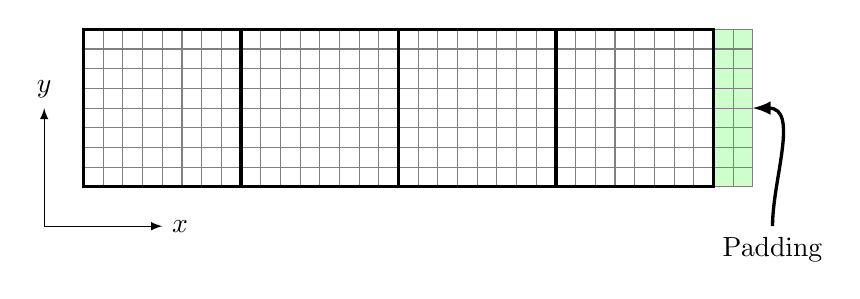
\begin{tikzpicture}[x=0.5cm,y=0.5cm]

\fill[green!20] (16,0) rectangle (17,4);
\draw[thin,gray,step=0.5] (0,0) grid (16,4);
\draw[thin,gray,step=0.5] (16,0) grid (17,4);
\draw[very thick,step=4] (0,0) grid (16,4);
\draw[very thick] (0,0) rectangle (16,4);

\coordinate (pad) at (17, 2);
\draw[-latex,very thick] (pad)+(0.5,-3) node[below]{Padding}
				to[out=90,in=0] (pad);

\coordinate (O) at (-1, -1, 0);
\draw[-latex] (O) -- +(3, 0,  0) node [right] {$x$};
\draw[-latex] (O) -- +(0,  3, 0) node [above] {$y$};
\end{tikzpicture}
\caption{A block divided in four regions, each corresponding to a plasma chunk.  
Extra padding is added at the right for internal use in the FFTW library.}
\label{fig:block}
\end{figure}%}}}

A simplified representation of a block can be observed in the 
figure~\ref{fig:block}, where the X dimension of each field is contiguous in 
memory.  Notice the padding region in green, which is needed for the FFTW 
library to store intermediate values. The use of ghost elements is needed for 
communications and will be detailed in the chapter~\ref{ch:comm}. If we look at 
each cell $(x,y)$ in the block we find the four components $\rho(x,y)$, 
$\phi(x,y)$, $E_x(x,y)$ and $E_y(x,y)$.

\section{Simulation flow}

The simulation follows a very precise set of steps to ensure the correct 
behavior of the physical simulation. Three main stages can be easily identified: 
Initialization, loop and finish.

\subsection{Initialization}

The iteration counter is initially set to $-2$, as we are going to do two 
previous phases before the simulation begins:

\paragraph{Allocation phase}
After $P$ processes were created (as in MPI processes), now we create the 
different structures to hold the simulation data. First the fields are 
distributed into task blocks, grouped in each process. For each specie, we 
distribute the particles based on the particle index $p_i$, minimizing the 
difference of the number of particles between blocks. The position, velocity and 
other parameters are set on each particle, independently of the actual block 
they reside.

Once all particles are initialized, we begin to move them to the correct block, 
based on the particle position, and increment the iteration counter. Finally, 
the charge density field $\rho$ is initially computed, as we want the begin the 
simulation with the computation of the electric field E from $\rho$

\paragraph{Rewind phase} The simulation time is not advanced equally for the 
speed and position of the particles. At time $t$ the velocity computed at time 
$t + \dt/2$ whereas the position is computed at time $t$. In order to begin the 
simulation, the velocity of the particles is advanced half time-step backwards 
in time. This extra step is computed at the iteration $i=-1$, as we need the 
iteration counter to be always increasing (as is used in the message exchange as 
unique identifier).

\subsection{Loop}

The loop of the simulation perform four main phases:

\begin{itemize}
\item Solve field equation to get $E$ from $\rho$.
\item Interpolate $E$ at particle positions $E_p$.
\item Particle motion based on $E_p$ and $B_0$.
\item Accumulate charge density $\rho$ at the new position of particles.
\end{itemize}

\subsubsection{Solver}

We use the MFT method to solve the equation:
\begin{equation}
\nabla^2 E = - \frac{\rho}{\epsilon_0}
\end{equation}

\subsection{Finish}

Here we hopefully save some information of the simulation to disk...

\section{Parallelization}

\subsection{Charge accumulation}

The interpolation process described in the equation~\ref{charge-accumulation} is 
executed in parallel for all the particles of each chunk. The charge density 
field is being updated in parallel, which involves the four surrounding grid 
points of a particle, and it may happen that at the frontier of two chunks a 
concurrent access to the same element occurs.

To avoid a race condition with the next chunk, a dependency is added with the 
directive \texttt{commutative}.

\begin{lstlisting}[caption={Task to update $\rho$ field using the 
\texttt{commutative} directive}, captionpos=b]
for (i=0; i<plasma->nchunks; i++)
{
	c0 = &plasma->chunks[i];
	c1 = &plasma->chunks[(i + 1) % plasma->nchunks];
	#pragma oss task commutative(*c0, *c1) label(rho_update_0)
	rho_update(sim, i);
}

\end{lstlisting}
